% 0167(본책 35쪽 · 배치 목록 빈틈, 쪽 이미지에서 전사) — 평행사변형 ABCD(AB=10cm, BC=11cm, ∠B=120°) 색칠. 스캔 삽화를 TikZ 로 다시 그림. 답(넓이)은 적지 않는다.
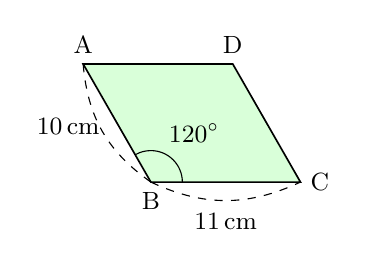
\begin{tikzpicture}[line width=0.6pt]
  \coordinate (B) at (0,0); \coordinate (C) at (1.9,0); \coordinate (A) at (-0.86,1.5); \coordinate (D) at (1.04,1.5);
  \fill[green!15] (A) -- (B) -- (C) -- (D) -- cycle;
  \draw (A) -- (B) -- (C) -- (D) -- cycle;
  \draw[line width=0.4pt] (0.4,0) arc[start angle=0, end angle=120, radius=0.4];
  \node[font=\small] at (0.55,0.62) {$120^\circ$};
  \draw[dashed, line width=0.4pt] (A) to[bend right=25] (B);
  \draw[dashed, line width=0.4pt] (B) to[bend right=25] (C);
  \node[font=\small] at (-1.05,0.7) {$10\,\mathrm{cm}$};
  \node[font=\small] at (0.95,-0.5) {$11\,\mathrm{cm}$};
  \node[font=\small, above] at (A) {A};
  \node[font=\small, below] at (B) {B};
  \node[font=\small, right] at (C) {C};
  \node[font=\small, above] at (D) {D};
\end{tikzpicture}
